\documentclass[letterpaper,openany,twoside,twocolumn]{book}
%\documentclass[a4paper,openany,oneside,twocolumn]{book}

\newcommand{\PATH}{../../}

\usepackage[justified]{\PATH dndtemplate/dnd}
\usepackage{\PATH monsters/stylesheets/monster_stylesheet}

\usepackage[english]{babel}
\usepackage[utf8]{inputenc}

%\newcommand{\entryfont}{\DndFontStatBlockBody} & uses the default font provided by the LaTeX DnD-Template
\newfontfamily\entryfont{Kalam}[Path=\PATH template/fonts/,Extension=.ttf,UprightFont=Kalam-Regular,BoldFont=Kalam-Bold] % requires XeLaTeX or LuaTeX

\begin{document}

%\layout

\MonsterSheetGeometry

\mainmatter%

% --------------------------------------------------------------------------------------------------- %
% ################################################################################################### %
% #-#-#-#-#-#-#-#-#-#-#-#-#-#-# Monster-Sheet with two Smaller Pictures #-#-#-#-#-#-#-#-#-#-#-#-#-#-# %
% ################################################################################################### %
% --------------------------------------------------------------------------------------------------- %

\MonsterFooterGraphic{0pt}% offset for text to bottom
	{250pt}% max height of the image
	{images/Magma_Turtle_Hatchling.png}% image to be displayed as a banner
	{}% used for keepaspectratio for image ({} or {, keepaspectratio})
	
\nopagebreaksection{\entryfont Magma Turtle}

\entryfont \noindent \DndDropCapLine{B}orn of elemental chaos and forged in the crucible of molten earth, the Magma Turtle emerges as a symbol of power and endurance. In its nature, the Magma Turtle maintains a neutral alignment, embodying the harmonious balance between opposing forces. These guardians of the elements exemplify the unbreakable bond between land and water, fire and earth. They stand as reminders of the raw power of nature, shaping and molding life in extraordinary ways. With their presence, they illuminate the delicate balance between fierce determination and graceful adaptation, a testament to the enduring spirit of the Magma Turtle. \\

\paragraph{Species Forms} The creation of these magnificent creatures is a marvel to behold. From humble hatchlings nestled in volcanic rock, their journey begins. The land-dwelling Magma Turtle, absorbing the scorching heat of its volcanic surroundings, grows in stature and resilience. The water-dwelling Magma Turtle, however, undergoes a metamorphosis, adapting to the depths near underwater volcanoes. It becomes reliant on the heat of the surrounding volcanic water, a lifeline for its survival.

In its land form, the Magma Turtle commands attention with its colossal presence. Its stone-hard shell, resembling solidified lava, radiates a fiery glow. With blazing determination in its eyes, it wields a formidable fiery tail club, delivering devastating blows to invaders and attackers. This symbol of power emits licking flames, a warning to those foolish enough to challenge its dominion. Born of fire and stone, the Magma Turtle stands as an indomitable force, ready to unleash its wrath upon any who threaten its realm.

In its water form, the Magma Turtle becomes a majestic ruler of the depths. Its shell, smooth like polished obsidian, reflects the allure of the underwater realm. Fiery luminescence traces sinuous lines on its surface, guiding its path through the watery abyss. With scalding streams of water gushing from its mouth, it repels invaders and attackers, defending its serene aquatic sanctuary. The Magma Turtle, embodying the convergence of fire and water, is a breathtaking sight beneath the waves, showcasing the boundless power and beauty that dwell in the depths.

\vfill\eject % cammand to break to next column

\vspace*{-3.6\fontdimen6\font}
% Monster stat block
\begin{DndMonster}[width=0.5\textwidth]{Magma Turtle (Hatchling)}
    \DndMonsterType{Tiny Elemental, neutral}

    % If you want to use commas in the key values, enclose the values in braces.
    \DndMonsterBasics[
        armor-class = {17 (natural armor)},
        hit-points  = {\DndDice{4d4 + 8}},
        speed       = {20 ft.},
    ]

    \DndMonsterAbilityScores[
        str = 8,
        dex = 13,
        con = 15,
        int = 2,
        wis = 12,
        cha = 7,
    ]

    \DndMonsterDetails[
        saving-throws = {Con +6},
        %skills = {Acrobatics +0, Animal Handling +0, Arcana +0, Athletics +0, Deception +0, History +0, Insight +0, Intimidation +0, Investigation +0, Medicine +0, Nature +0, Perception +0, Performance +0, Persuasion +0, Religion +0, Sleight of Hand +0, Stealth +0, Survival +0},
        damage-vulnerabilities = {cold},
        damage-resistances = {bludgeoning, piercing, and slashing from nonmagical attacks},
        damage-immunities = {fire},
        senses = {Darkvision 60ft., Passive Perception 11},
        condition-immunities = {exhaustion, paralyzed, petrified, poisoned},
        languages = {understands Primordial but can't speak},
        challenge = 1/2,
    ]
    
    \DndMonsterAction{Fire Vulnerability}
    For every 5ft. the Magma Turtle (Hatchling) moves through water or for each each gallon of water splashed on it, it takes 1 cold damage.
    
    \DndMonsterAction{Molten Rock Shell}
    The Magma Turtle Hatchling's shell provides it with resistance to bludgeoning, piercing, and slashing damage from nonmagical attacks.
	
	\DndMonsterSection{Actions}
	
	\DndMonsterAttack[
      name=Bite,
      distance=melee, % valid options are in the set {both,melee,ranged},
      %type=weapon, %valid options are in the set {weapon,spell}
      mod=+1,
      reach=5,
      %range=20/60,
      targets=one target,
      dmg=\DndDice{1d4 + 1},
      dmg-type=piercing,
      %plus-dmg=,
      %plus-dmg-type=,
      %or-dmg=,
      %or-dmg-when=,
      %extra=,
    ]
      
\end{DndMonster}

The Magma Turtle (Hatchling) is a mesmerizing creature, embodying the essence of fire and stone. It is a small marvel, with a robust and stone-hard shell resembling the solidified form of molten lava. Adorned with intricate and glowing cracks, the shell emits a vibrant red glow, casting an otherworldly radiance upon the surrounding landscape. Agile and resilient, the hatchling scampers with surprising grace across rocky terrains near underwater volcanoes, absorbing the intense heat of its environment. Its fiery eyes, shimmering with determination, surveil the land, ever watchful for potential threats and sources of warmth.

The hatchling's compact frame and formidable shell display the seeds of its future power. With each passing day, it grows stronger and more resilient, harnessing the energy of its volcanic home. It is a creature on the cusp of transformation, destined to become a mighty Magma Turtle. In its presence, one can sense the latent power and untamed potential, foretelling a future where this small and captivating hatchling will emerge as a force to be reckoned \blocktextlinebreak\hspace*{2.4cm} with, navigating the land and water with \blocktextlinebreak\hspace*{3.6cm} unmatched strength and endurance.

\newpage

\begin{tikzpicture}[overlay, remember picture, inner sep=0pt, outer sep=0pt, path fading=fade down]%
	\node (posN) at (current page text area.north) {};%
	\node[above left=20pt and 5.75cm of posN, anchor=north] (cornerNW) {%
		\begin{minipage}{\columnwidth}%%
        	\centering\includegraphics[width=1.1\columnwidth, height=280pt, keepaspectratio]{images/Magma_Turtle_Waterform.png}%
      	\end{minipage}%
	};%
\end{tikzpicture}%

\hfill\\\vspace*{1.75cm}

% Monster stat block
\begin{DndMonster}[width=0.5\textwidth]{Magma ~~~~~~~~~~~~~~ Turtle\\(Waterform)}
    \DndMonsterType{Large Elemental, neutral}

    % If you want to use commas in the key values, enclose the values in braces.
    \DndMonsterBasics[
        armor-class = {18 (natural armor)},
        hit-points  = {\DndDice{12d10 + 60}},
        speed       = {10 ft., 60 ft. swim},
    ]

    \DndMonsterAbilityScores[
        str = 14,
        dex = 14,
        con = 20,
        int = 6,
        wis = 12,
        cha = 8,
    ]

    \DndMonsterDetails[
        saving-throws = {Dex +4, Con +7},
        skills = {Perception +4},
        %damage-vulnerabilities = {Fire},
        damage-resistances = {Bludgeoning, Piercing, and Slashing from Nonmagical Attacks},
        damage-immunities = {Fire},
        senses = {Darkvision 60ft, Passive Perception 14},
        condition-immunities = {Petrified},
        languages = {Primordial},
        challenge = 7,
    ]
    
	\DndMonsterAction{Amphibious}
	The Magma Turtle can breathe air and water.
	
	\DndMonsterAction{Keen Smell}
	The Magma Turtle has advantage on Wisdom (Perception) checks that rely on smell.
    
    \DndMonsterAction{Molten Rock Shell}
    The Magma Turtle Hatchling's shell provides it with resistance to bludgeoning, piercing, and slashing damage from nonmagical attacks.
	
	\DndMonsterSection{Actions}
	
	\DndMonsterAction{Multiattack}
	The Magma Turtle (Waterform) can make one Pound Attack and one Fiery Stream Attack on each of its turns.
	
	\DndMonsterAttack[
      name=Pound,
      distance=melee, % valid options are in the set {both,melee,ranged},
      %type=weapon, %valid options are in the set {weapon,spell}
      mod=+7,
      reach=5,
      %range=20/60,
      targets=one target,
      dmg=\DndDice{2d8 + 5},
      dmg-type=bludgeoning,
      %plus-dmg=,
      %plus-dmg-type=,
      %or-dmg=,
      %or-dmg-when=,
      %extra=,
    ]
    
    \DndMonsterAction{Fiery Streams}
	The Magma Turtle can unleash hot streams of water as a ranged spell attack (+4 to hit, 20/60 ft. range). All targets in the line of effect must make a DC 15 Dexterity saving throw taking 4d8 fire damage on a failed one, or half damage on a successful save.
    
    \DndMonsterSection{Reactions}
    
    \DndMonsterAction{Shell Defense}
    When the Magma Turtle is hit by a melee attack, it can use its reaction to retract into its shell, gaining a +4 bonus to its AC until the start of its next turn.
      
\end{DndMonster}

\vfill\eject % command to break to next column

% Monster stat block
\begin{DndMonster}[width=0.5\textwidth +0.5em]{Magma Turtle (Landform)}
    \DndMonsterType{Large Elemental, neutral}

    % If you want to use commas in the key values, enclose the values in braces.
    \DndMonsterBasics[
        armor-class = {16 (natural armor)},
        hit-points  = {\DndDice{16d10 + 48}},
        speed       = {20 ft.},
    ]

    \DndMonsterAbilityScores[
        str = 20,
        dex = 12,
        con = 16,
        int = 10,
        wis = 14,
        cha = 10,
    ]

    \DndMonsterDetails[
        %saving-throws = {Str +0, Dex +0, Con +0, Int +0, Wis +0, Cha +0},
        skills = {Perception +6},
        damage-vulnerabilities = {Fire},
        %damage-resistances = {bludgeoning, piercing, and slashing from nonmagical attacks},
        damage-immunities = {Exhaustion, Frightened, Poisoned},
        senses = {Darkvision 60ft, passive Perception 15},
        %condition-immunities = {frightened, poisoned},
        languages = {Sylvan},
        challenge = 8,
    ]
    
    \DndMonsterAction{Photosynthesis}
    Whenever the Grove Sentinel (Strength) is ending its turn in direct sunlight, it regains \DndDice{2d6} hitpoints.
    
	\DndMonsterAction{Mighty Strikes}
	The Grove Sentinel's melee (Strength) weapon attacks deal an extra \DndDice{2d6} damage.
    
    \DndMonsterAction{Crushing Roots}
    When the Grove Sentinel (Strength) hits a creature with a melee attack, it can use its reaction to summon thick roots from the ground to restrain the target. The restrained creature must succeed on a DC 15 Strength saving throw or be restrained until the start of its next turn. The creature can use its action to make a DC 15 Strength check, freeing itself or another creature within its reach on a success. The effect ends if the roots are destroyed (AC 15, 10 hit points, vulnerability to fire damage).
     
     \DndMonsterAction{Enhanced Regeneration}
     At the start of its turn, the Grove Sentinel (Strength) regains \DndDice{1d12} hit points.
	
	\DndMonsterSection{Actions}
	
	\DndMonsterAction{Multiattack}
	The Grove Sentinel (Strength) makes two slam attacks.
	
	\DndMonsterAttack[
      name=Slam,
      distance=melee, % valid options are in the set {both,melee,ranged},
      %type=weapon, %valid options are in the set {weapon,spell}
      mod=+9,
      reach=10,
      %range=20/60,
      targets=one target,
      dmg=\DndDice{2d6 + 5},
      dmg-type=bludgeoning,
      %plus-dmg=,
      %plus-dmg-type=,
      %or-dmg=,
      %or-dmg-when=,
      %extra=,
    ]
    
    \DndMonsterAction{Rending Smash}
    The Grove Sentinel (Strength) delivers a devastating pounce empowered by its immense strength. The Sentinel makes a single slam attack against a target. On a hit, the target takes an additional 10 (3d6) bludgeoning damage and must succeed on a DC 15 Strength saving throw or have its movement speed reduced by half until the start of its next turn.
    
    \DndMonsterAction{Ground Shatter (Recharge 5-6)}
	The Grove Sentinel (Strength) slams the ground with immense force, causing a shockwave in a 20-foot radius centered on itself. Each creature in that area must make a DC 15 Dexterity saving throw, taking \DndDice{7d6} force damage on a failed save, or half as much damage on a successful one.
      
\end{DndMonster}

\begin{tikzpicture}[overlay, remember picture, inner sep=0pt, outer sep=0pt, path fading=fade down]%
	\node (posN) at (current page text area.north) {};%
	\node[above left=20pt and 5.75cm of posN, anchor=north] (cornerNW) {%
		\begin{minipage}{\columnwidth}%%
        	\centering\includegraphics[width=1.1\columnwidth, height=280pt, keepaspectratio]{images/Magma_Turtle_Waterform_above.png}%
      	\end{minipage}%
	};%
\end{tikzpicture}%

\begin{tikzpicture}[overlay, remember picture, inner sep=0pt, outer sep=0pt, path fading=fade down]%
	\node (posS) at (current page text area.south) {};%
	\node[below right=0pt and 5cm of posS, anchor=south] (cornerSE) {%
		\begin{minipage}{\columnwidth}%%
        	\centering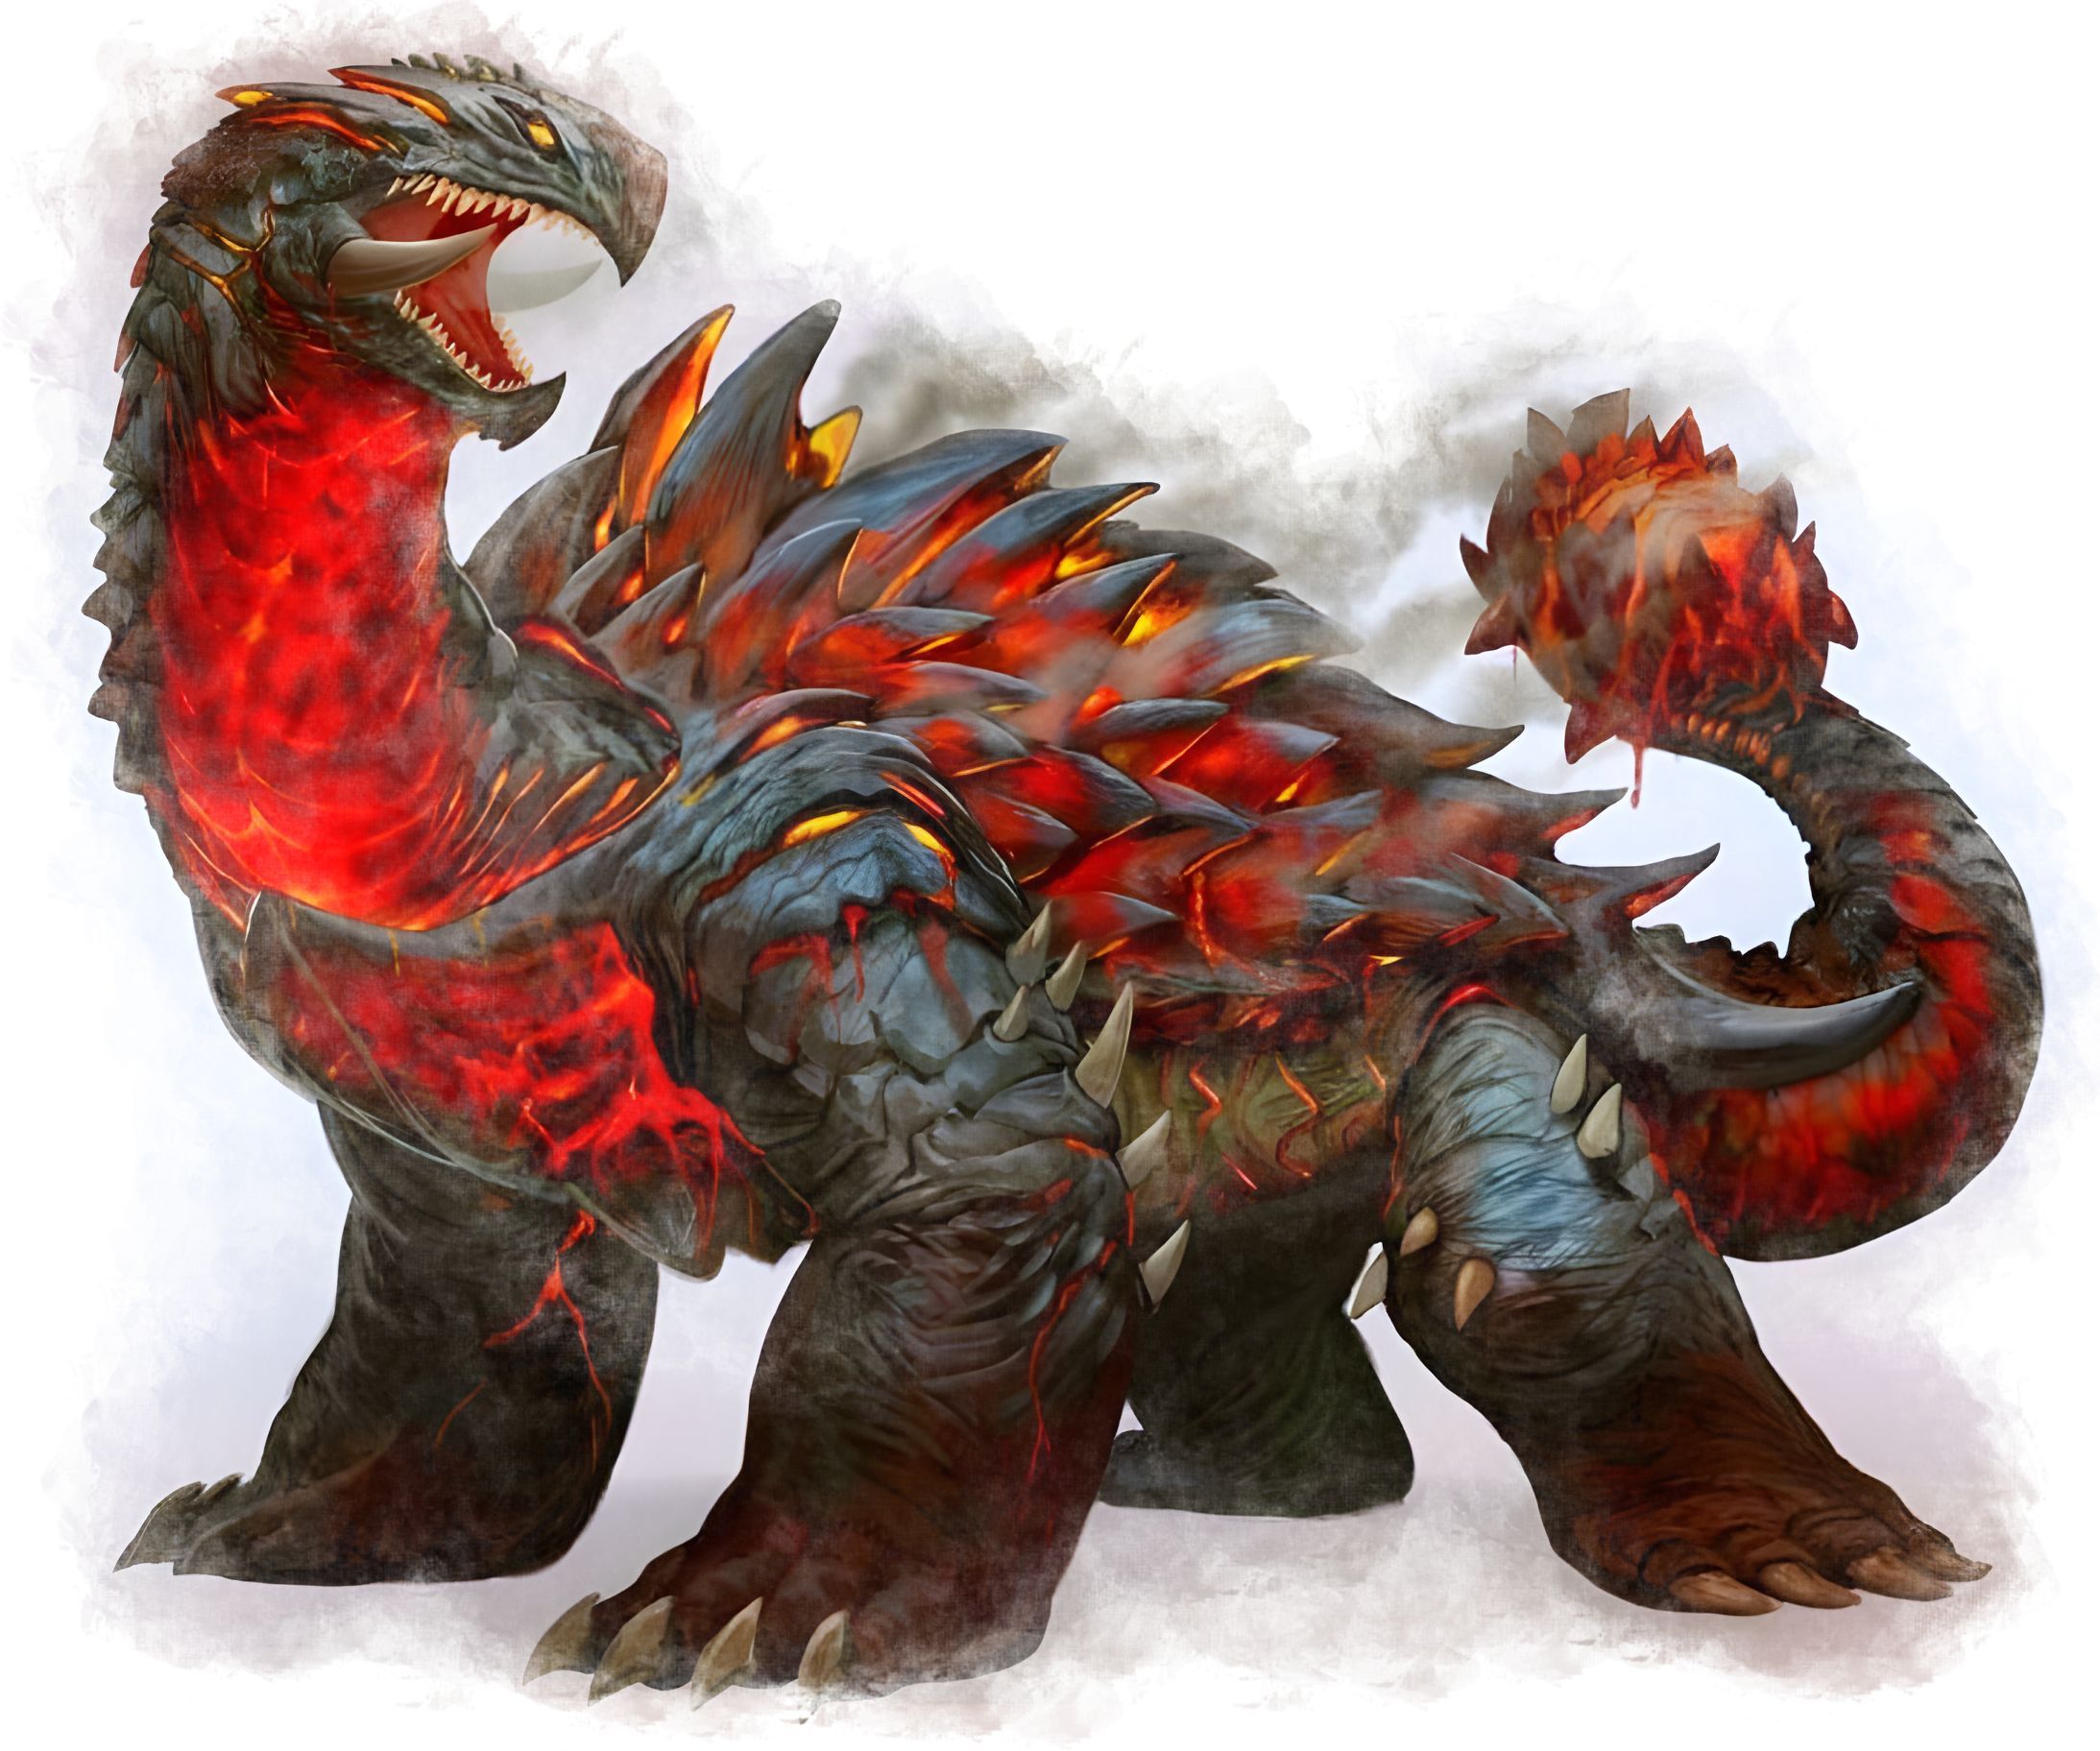
\includegraphics[width=1.3\columnwidth, height=210pt, keepaspectratio]{images/Magma_Turtle_Landform.png}%
      	\end{minipage}%
	};%
\end{tikzpicture}%

\end{document}
